\pdfminorversion=7
\documentclass[11pt,letterpaper]{article}

\usepackage[utf8]{inputenc}
\usepackage[T1]{fontenc}
\usepackage[french]{babel}
\frenchsetup{SmallCapsFigTabCaptions=false}
\usepackage[scale=0.95]{tgheros}
\renewcommand{\familydefault}{\sfdefault}
\usepackage{geometry}
\usepackage{graphicx}
\usepackage{grffile}
\usepackage{float}
\usepackage{booktabs}
\usepackage{longtable}
\usepackage{array}
\usepackage{tabularx}
\usepackage{xcolor}
\usepackage{tikz}
\usepackage{eso-pic}
\usepackage{fancyhdr}
\usepackage{titlesec}
\usepackage[font=small,labelfont=bf]{caption}
\usepackage{microtype}
\usepackage{indentfirst}
\usepackage{hyperref}

% Les ressources externes du dossier restent dans ces deux dossiers.
\graphicspath{{assets/}{img/}}

\geometry{
    letterpaper,
    left=0.95in,
    right=0.95in,
    top=1.55in,
    bottom=0.78in,
    headheight=18pt,
    headsep=18pt,
    footskip=28pt
}

\definecolor{tameoBlue}{HTML}{173B5C}
\definecolor{tameoLink}{HTML}{3A6B78}
\definecolor{tameoText}{HTML}{13283A}
\newcommand{\tameoCoverIndent}{0.20in}

\newcommand{\tameoTitle}{Bateau IA -- Groupe 25}
\newcommand{\tameoDocumentType}{Dossier de réalisation}
\newcommand{\tameoPdfTitle}{Dossier de réalisation du projet TAMEO-IA}
\newcommand{\tameoPdfAuthor}{Projet TAMEO-IA}

\newcommand{\tameoAuthorsBlockA}{%
    \tameoAuthorCell{CAVALLARO}{Vinicius Cesar}{vinicius-cesar.cavallaro@ensta.fr}
    & \tameoAuthorCell{COUERRE}{Loup}{loup.couerre@ensta.fr}
    \tabularnewline[0.56in]
    \tameoAuthorCell{DIAS LEITE}{Julia Ellen}{julia-ellen.dias@ensta.fr}
    & \tameoAuthorCell{MARCHÉ}{Benoît}{benoit.marche@ensta.fr}
}

\newcommand{\tameoAuthorsBlockB}{%
    \tameoAuthorCell{DA SILVEIRA}{Lucas}{lucas.da-silveira-absalao@ensta.fr}
    & \tameoAuthorCell{DE SOUZA AMODIO}{Lucca}{lucca.de-souza-amodio@ensta.fr}
    \tabularnewline[0.56in]
    \tameoAuthorCell{NOUKOUA TATMFO}{Maeva sandy}{maeva-sandy.noukoua@ensta.fr}
    & \tameoAuthorCell{TARAZONA JIMENEZ}{Javier andres}{javier-andres.tarazona@ensta.fr}
}

\hypersetup{
    colorlinks=true,
    linkcolor=tameoBlue,
    urlcolor=tameoLink,
    pdftitle={\tameoPdfTitle},
    pdfauthor={\tameoPdfAuthor}
}

\setlength{\parindent}{1.5em}
\setlength{\parskip}{0.35em}
\renewcommand{\arraystretch}{1.18}
\newcolumntype{L}[1]{>{\raggedright\arraybackslash}p{#1}}
\newcolumntype{Y}{>{\raggedright\arraybackslash}X}
\setlength{\emergencystretch}{1.5em}

\titleformat{\section}
  {\sffamily\bfseries\LARGE\color{tameoBlue}}
  {\thesection}{0.75em}{}
\titleformat{\subsection}
  {\sffamily\bfseries\large\color{tameoBlue}}
  {\thesubsection}{0.75em}{}
\titlespacing*{\section}{0pt}{1.3em}{0.65em}
\titlespacing*{\subsection}{0pt}{1.05em}{0.35em}

\pagestyle{fancy}
\fancyhf{}
\renewcommand{\headrulewidth}{0pt}
\fancyfoot[R]{\thepage}

\newcommand{\tameoBranding}{%
    \begin{tikzpicture}[remember picture,overlay]
        \node[anchor=north east] at ([xshift=-1.16in,yshift=-0.58in]current page.north east)
            {
\includegraphics[width=1.98in]{tameo-logo.png}};
        \node[anchor=north east] at ([xshift=-1.18in,yshift=-1.12in]current page.north east)
            {
\includegraphics[width=2.05in,height=0.026in]{tameo-bar.png}};
    \end{tikzpicture}%
}

\newcommand{\tameoAuthorCell}[3]{%
    \begin{minipage}[t]{2.6in}
        \raggedright
        \hyphenpenalty=10000
        \exhyphenpenalty=10000
        {\sffamily\fontsize{10.8}{12.6}\selectfont #1\par}
        {\sffamily\fontsize{10.2}{12}\selectfont #2\par}
        {\sffamily\fontsize{6.45}{7.6}\selectfont\href{mailto:#3}{#3}\par}
    \end{minipage}%
}

\newcommand{\maketameotitle}{%
    \begin{titlepage}
        \thispagestyle{empty}
        \begin{tikzpicture}[remember picture,overlay]
            \node[anchor=north east] at ([xshift=-1.37in,yshift=-2.42in]current page.north east)
                {
\includegraphics[width=1.82in]{tameo-logo.png}};
            \node[anchor=north west] at ([xshift=1.16in,yshift=-3.00in]current page.north west)
                {
\includegraphics[width=6.55in,height=0.115in]{tameo-bar.png}};
        \end{tikzpicture}

        \vspace*{1.82in}
        {\hspace*{\tameoCoverIndent}\sffamily\bfseries\fontsize{42}{50}\selectfont\color{tameoBlue}\tameoTitle\par}
        \vspace{0.45in}
        {\hspace*{\tameoCoverIndent}\sffamily\itshape\fontsize{16}{20}\selectfont\color{tameoText}\tameoDocumentType\par}

        \vspace{0.46in}
        \noindent\hspace*{\tameoCoverIndent}\makebox[0pt][l]{%
            \begin{tabular*}{5.95in}{@{\extracolsep{\fill}}ll@{}}
                \tameoAuthorsBlockA
            \end{tabular*}%
        }\par
        \vspace{0.25in}
        \noindent\hspace*{\tameoCoverIndent}\makebox[0pt][l]{%
            \begin{tabular*}{5.95in}{@{\extracolsep{\fill}}ll@{}}
                \tameoAuthorsBlockB
            \end{tabular*}%
        }
    \end{titlepage}
}

\makeatletter
\newcommand{\styledtableofcontents}{%
    \thispagestyle{fancy}
    \vspace*{1.05in}
    {\sffamily\bfseries\fontsize{24}{29}\selectfont\color{tameoBlue}Table des matières\par}
    \vspace{0.85in}
    \begingroup
    \parskip=0.18em
    \@starttoc{toc}
    \endgroup
    \newpage
}
\makeatother

\begin{document}

\maketameotitle
\setcounter{page}{2}
\AddToShipoutPictureBG{\tameoBranding}
\styledtableofcontents

\section{Introduction générale}

Le projet PIE TAMEO-IA s'inscrit dans le cadre de l'association TAMEO. Son objectif est d'apporter un support technique à la conception d'un bateau autonome destiné à participer à la classe IA du Monaco Energy Boat Challenge. Le projet vise à développer une architecture capable de percevoir l'environnement maritime, de produire des consignes de navigation et de contrôler le bateau pendant les différentes épreuves.

Le bateau final étant conçu et construit en parallèle du développement logiciel, l'équipe a utilisé une plateforme marine existante, le BlueBoat de Blue Robotics, comme banc d'essai. Ce support a permis de tester les codes d'intelligence artificielle, les éléments d'intégration, les communications et certains composants réels sans attendre la disponibilité complète du châssis final. Le BlueBoat a donc joué un rôle central : il a permis de valider progressivement les choix logiciels et matériels, de sécuriser les essais et de préparer la transition vers le bateau destiné à Monaco.

Dès le début du projet, une contrainte importante a été identifiée : l'accès tardif au châssis physique du bateau final. Les efforts ont donc été orientés vers la viabilité de la transition entre les fonctionnalités développées sur le BlueBoat et le prototype réel. Ce choix a évité de bloquer les pôles logiciels et a rendu possible le développement en parallèle de la vision, de la communication, de l'intégration des actionneurs, des capteurs et des procédures de test.

Le projet a également dû s'adapter à l'évolution des exigences de l'organisation du challenge. La question de la présence ou non d'un pilote à bord a évolué au cours de l'année, ce qui a eu un impact direct sur la configuration du châssis, la radiocommande, les modes de reprise en main et la conformité réglementaire.

\section{Organisation du projet}

Le travail a été réparti en plusieurs pôles complémentaires. Le pôle Vision a travaillé sur la reconnaissance des éléments utiles à la navigation, notamment les bouées fixes, les bouées mobiles et les repères de docking. Le pôle Navigation et trajectoire avait pour rôle de fournir une trajectoire en fonction des obstacles reconnus et de l'épreuve envisagée. Le pôle Simulation devait créer un jumeau numérique du bateau afin de visualiser et valider les actions de l'IA. Le pôle Tests et intégration s'est concentré sur la prise en main du BlueBoat, les essais réels et l'intégration sécurisée des composants. Enfin, les travaux de conception du bateau réel et de gestion technique ont assuré la cohérence matérielle, réglementaire et logistique du projet.

Dans cette organisation, les rôles se sont fortement recoupés autour du BlueBoat. Celui-ci a servi à la fois de plateforme de test pour la vision, de support d'intégration pour la Jetson et les caméras, de moyen de validation des communications MAVLink, et de banc de pré-intégration pour des composants destinés au bateau final.

Les principales contributions couvertes par ce dossier sont les suivantes :

\begin{itemize}
    \item mise en place d'un pipeline de vision complet, depuis la collecte de données jusqu'à l'entraînement et l'inférence ;
    \item intégration de la Jetson, des caméras, d'un switch réseau et des accès distants sur le BlueBoat ;
    \item étude et validation de l'architecture BlueOS, ArduPilot, MAVLink et QGroundControl ;
    \item adaptation de la communication avec les contrôleurs moteurs VESC ;
    \item conception de bancs de test pour les moteurs, la direction, le GPS et la radiocommande ;
    \item contribution à la conception globale du bateau réel, de son système électrique et de son système de direction ;
    \item suivi de la conformité réglementaire, des commandes, du budget et de la disponibilité des composants.
\end{itemize}

\section{Plateforme BlueBoat et environnement de test}

\subsection{Rôle du BlueBoat}

Le BlueBoat est une plateforme marine développée par Blue Robotics. Il peut être contrôlé depuis une station à terre par Wi-Fi et dispose de son propre système d'exploitation, BlueOS. Il repose sur une variante d'ArduPilot, ce qui permet d'utiliser des outils classiques de contrôle de vol et de planification de mission.

Dans le cadre du projet, le BlueBoat a été modifié pour devenir un banc d'essai du système autonome. Il a permis de tester les codes d'IA et d'intégration avant la disponibilité complète du bateau final. Cette approche a été particulièrement utile pour conserver un rythme de développement malgré les contraintes matérielles et l'accès limité à des plans d'eau.

\begin{figure}[H]
    \centering
    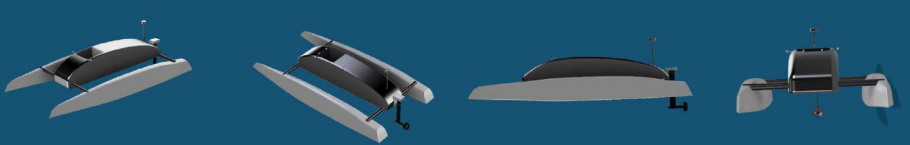
\includegraphics[width=0.85\linewidth]{blueboat.png}
    \caption{Plateforme BlueBoat utilisée comme support de développement et de test.}
\end{figure}

\subsection{Prise en main logicielle}

La prise en main du BlueBoat a nécessité l'étude de sa documentation, de son interface BlueOS et de ses modes de contrôle. L'équipe a choisi d'utiliser QGroundControl afin de disposer d'un affichage en temps réel de la position du bateau et de pouvoir changer rapidement de mode de fonctionnement. Ce point était essentiel pour tester des fonctions autonomes tout en conservant une capacité de reprise en main rapide en cas de défaillance de la partie IA.

\begin{figure}[H]
    \centering
    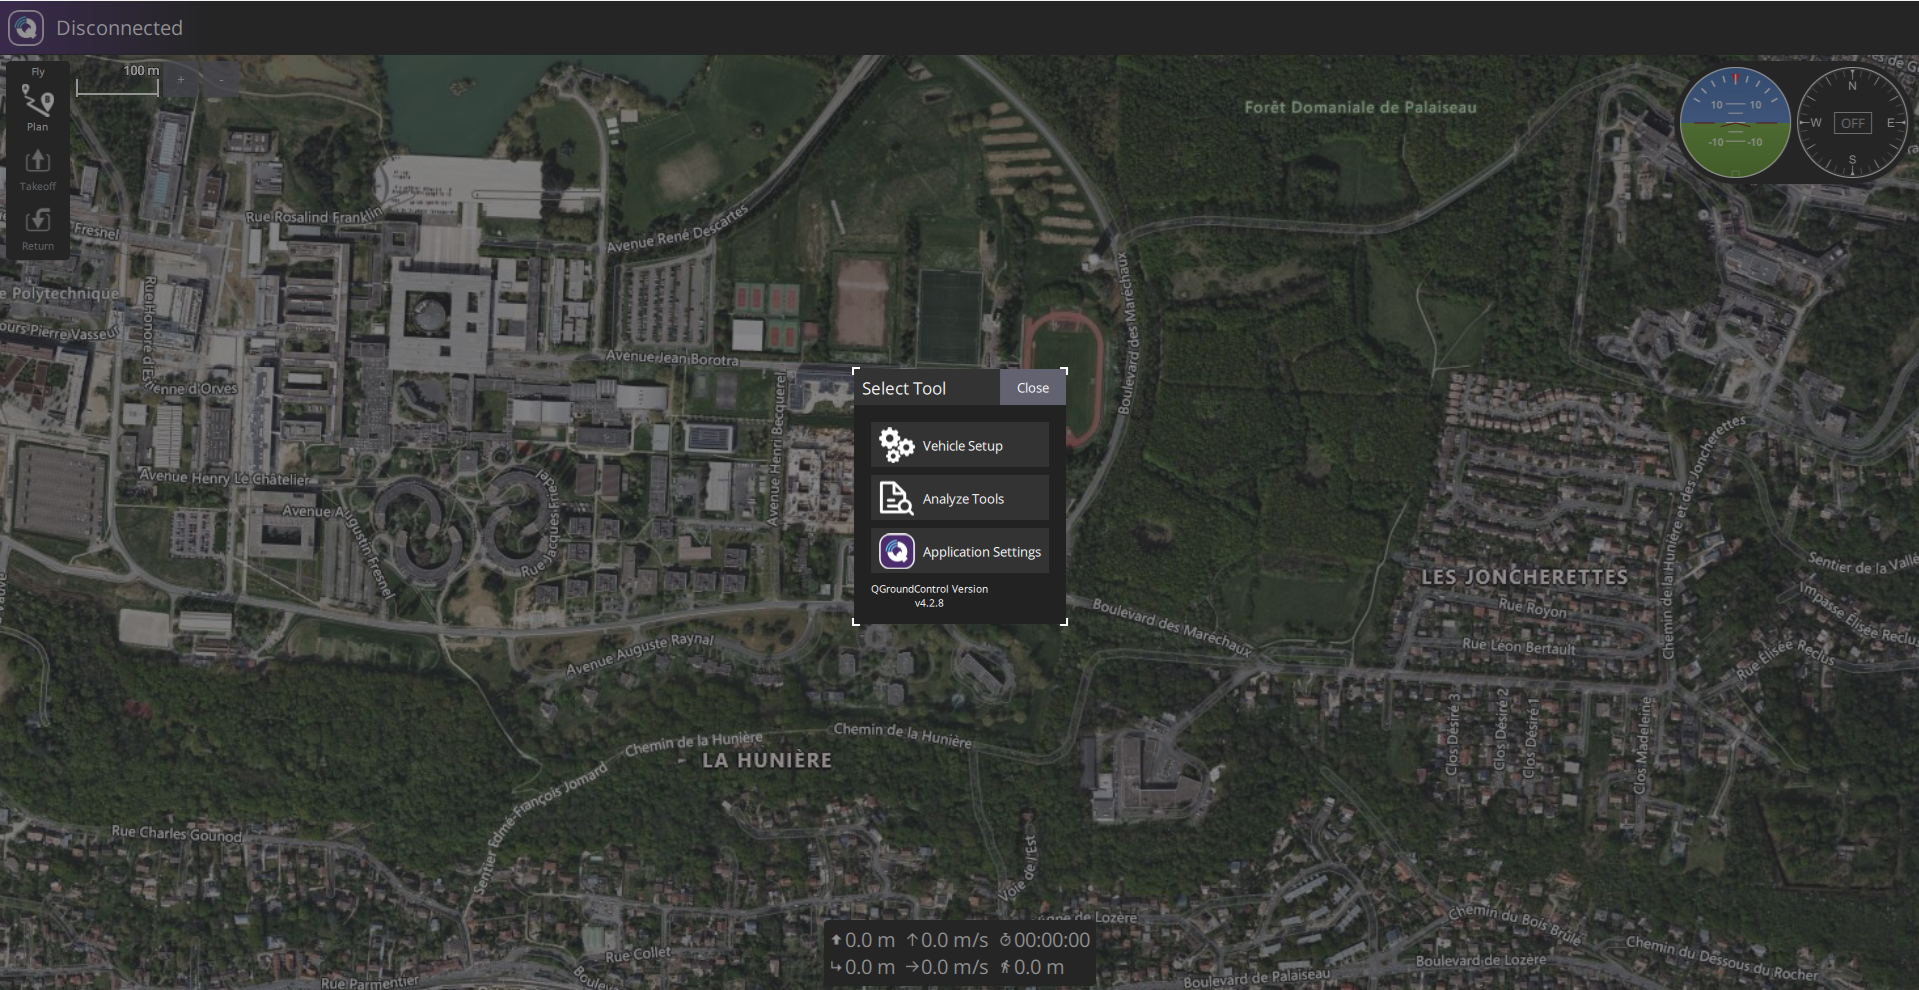
\includegraphics[width=0.9\linewidth]{qgc.png}
    \caption{Interface QGroundControl utilisée pour suivre la position du bateau et gérer ses modes de fonctionnement.}
\end{figure}

L'interface web BlueOS est accessible lorsque l'on est connecté au réseau local du BlueBoat, notamment via \texttt{blueos.local} ou l'adresse \texttt{192.168.2.2}. Elle permet de visualiser les messages MAVLink échangés entre les composants, de modifier certains paramètres de l'autopilote, comme le mapping des moteurs ou l'utilisation d'interfaces, et d'accéder à des fonctions avancées. Les modifications de paramètres restent toutefois limitées aux plages autorisées par ArduPilot, ce qui a constitué une contrainte lors de l'intégration de composants non prévus par défaut.

Le mode pirate de BlueOS permet d'atteindre des fonctions plus avancées, par exemple la modification de l'arborescence de fichiers ou la création d'interfaces MAVLink avec de nouveaux composants. Cette possibilité a été utilisée dans la réflexion sur l'intégration de l'ordinateur embarqué et des contrôleurs moteurs.

\subsection{Architecture réseau et accès distants}

L'ajout de la Jetson et des caméras a imposé une modification de l'architecture réseau. La communication devait être assurée simultanément entre le BlueBoat, la Jetson et un ordinateur à terre. L'ordinateur à terre devait pouvoir superviser le système, récupérer des données et reprendre le contrôle du bateau si nécessaire.

Pour répondre à ce besoin, un switch Ethernet embarqué a été ajouté. Il permet d'intégrer la Jetson au réseau local sans détruire l'architecture initiale du BlueBoat. Une adresse IP statique de la Jetson a également été ajoutée aux endpoints MAVLink de BlueOS afin de pouvoir envoyer des commandes MAVLink directes depuis Python.

\begin{figure}[H]
    \centering
    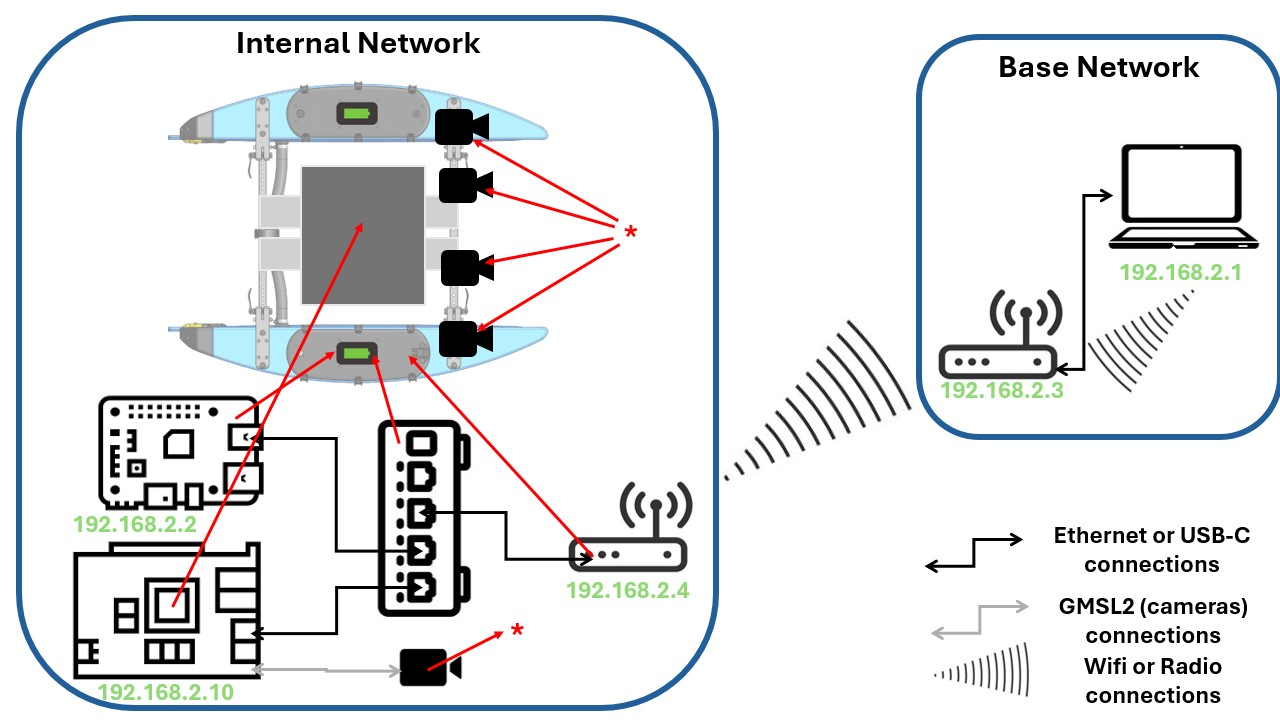
\includegraphics[width=0.9\linewidth]{architecture-blueboat.jpg}
    \caption{Architecture réseau mise en place autour du BlueBoat, de la Jetson et de la station à terre.}
\end{figure}

Cette architecture permet d'utiliser la station de base et le réseau interne du BlueBoat pour se connecter à distance à la Jetson, par exemple en SSH ou avec un client VNC comme RealVNCViewer.

\begin{figure}[H]
    \centering
    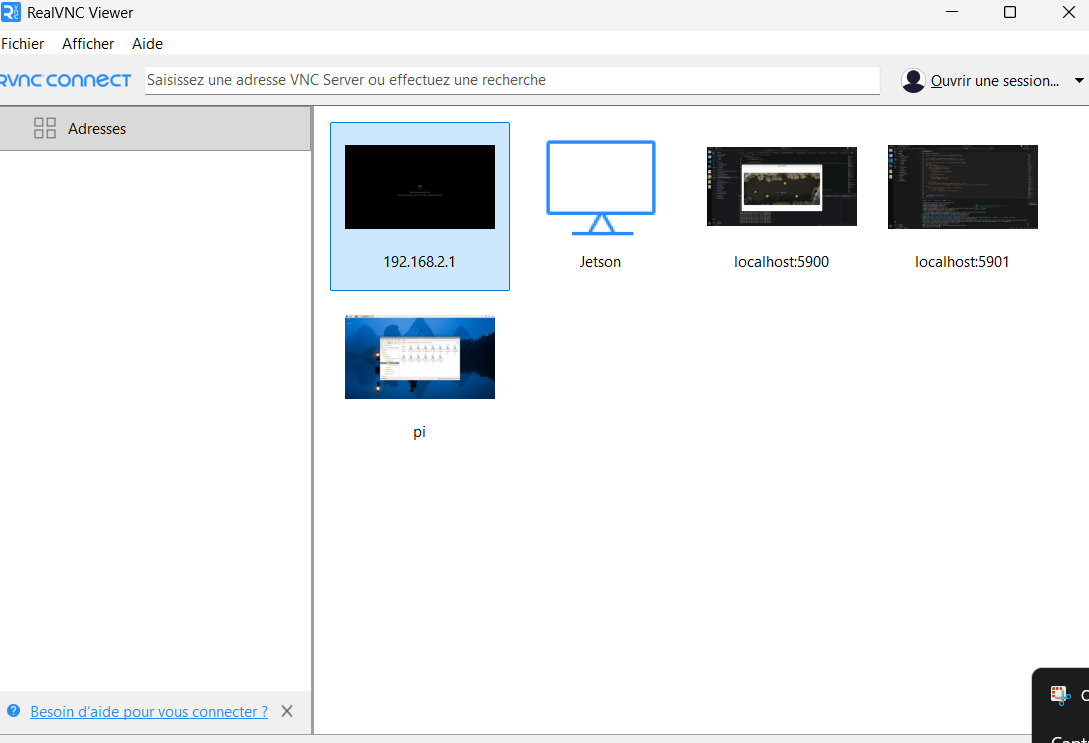
\includegraphics[width=0.8\linewidth]{vnc.png}
    \caption{Connexion distante à l'environnement embarqué.}
\end{figure}

\subsection{Intégration physique de la Jetson et des caméras}

L'intégration d'un module de calcul embarqué NVIDIA Jetson avait pour objectif de fournir la puissance nécessaire au traitement des données capteurs et au pilotage autonome du bateau. La Jetson devait pouvoir exploiter les caméras embarquées et participer à la gestion de la trajectoire en temps réel.

Sur le plan mécanique, une boîte étanche a été conçue et fixée sur le bateau pour accueillir la Jetson. Cette boîte a été pensée pour rester mobile afin de permettre l'ajustement du centre de gravité du bateau, point important pour garantir sa stabilité. Les caméras ont été fixées à l'avant du bateau pour optimiser leur champ de vision dans les futures applications de perception.

L'intégration a aussi nécessité un travail de câblage électrique. L'objectif était d'assurer une alimentation fiable et sécurisée de la Jetson à partir des batteries du BlueBoat, tout en respectant les contraintes d'intégration et de sécurité. Ce travail a abouti à un système fonctionnel, prêt à être utilisé pour les phases de test et de développement des fonctions autonomes.

\begin{figure}[H]
    \centering
    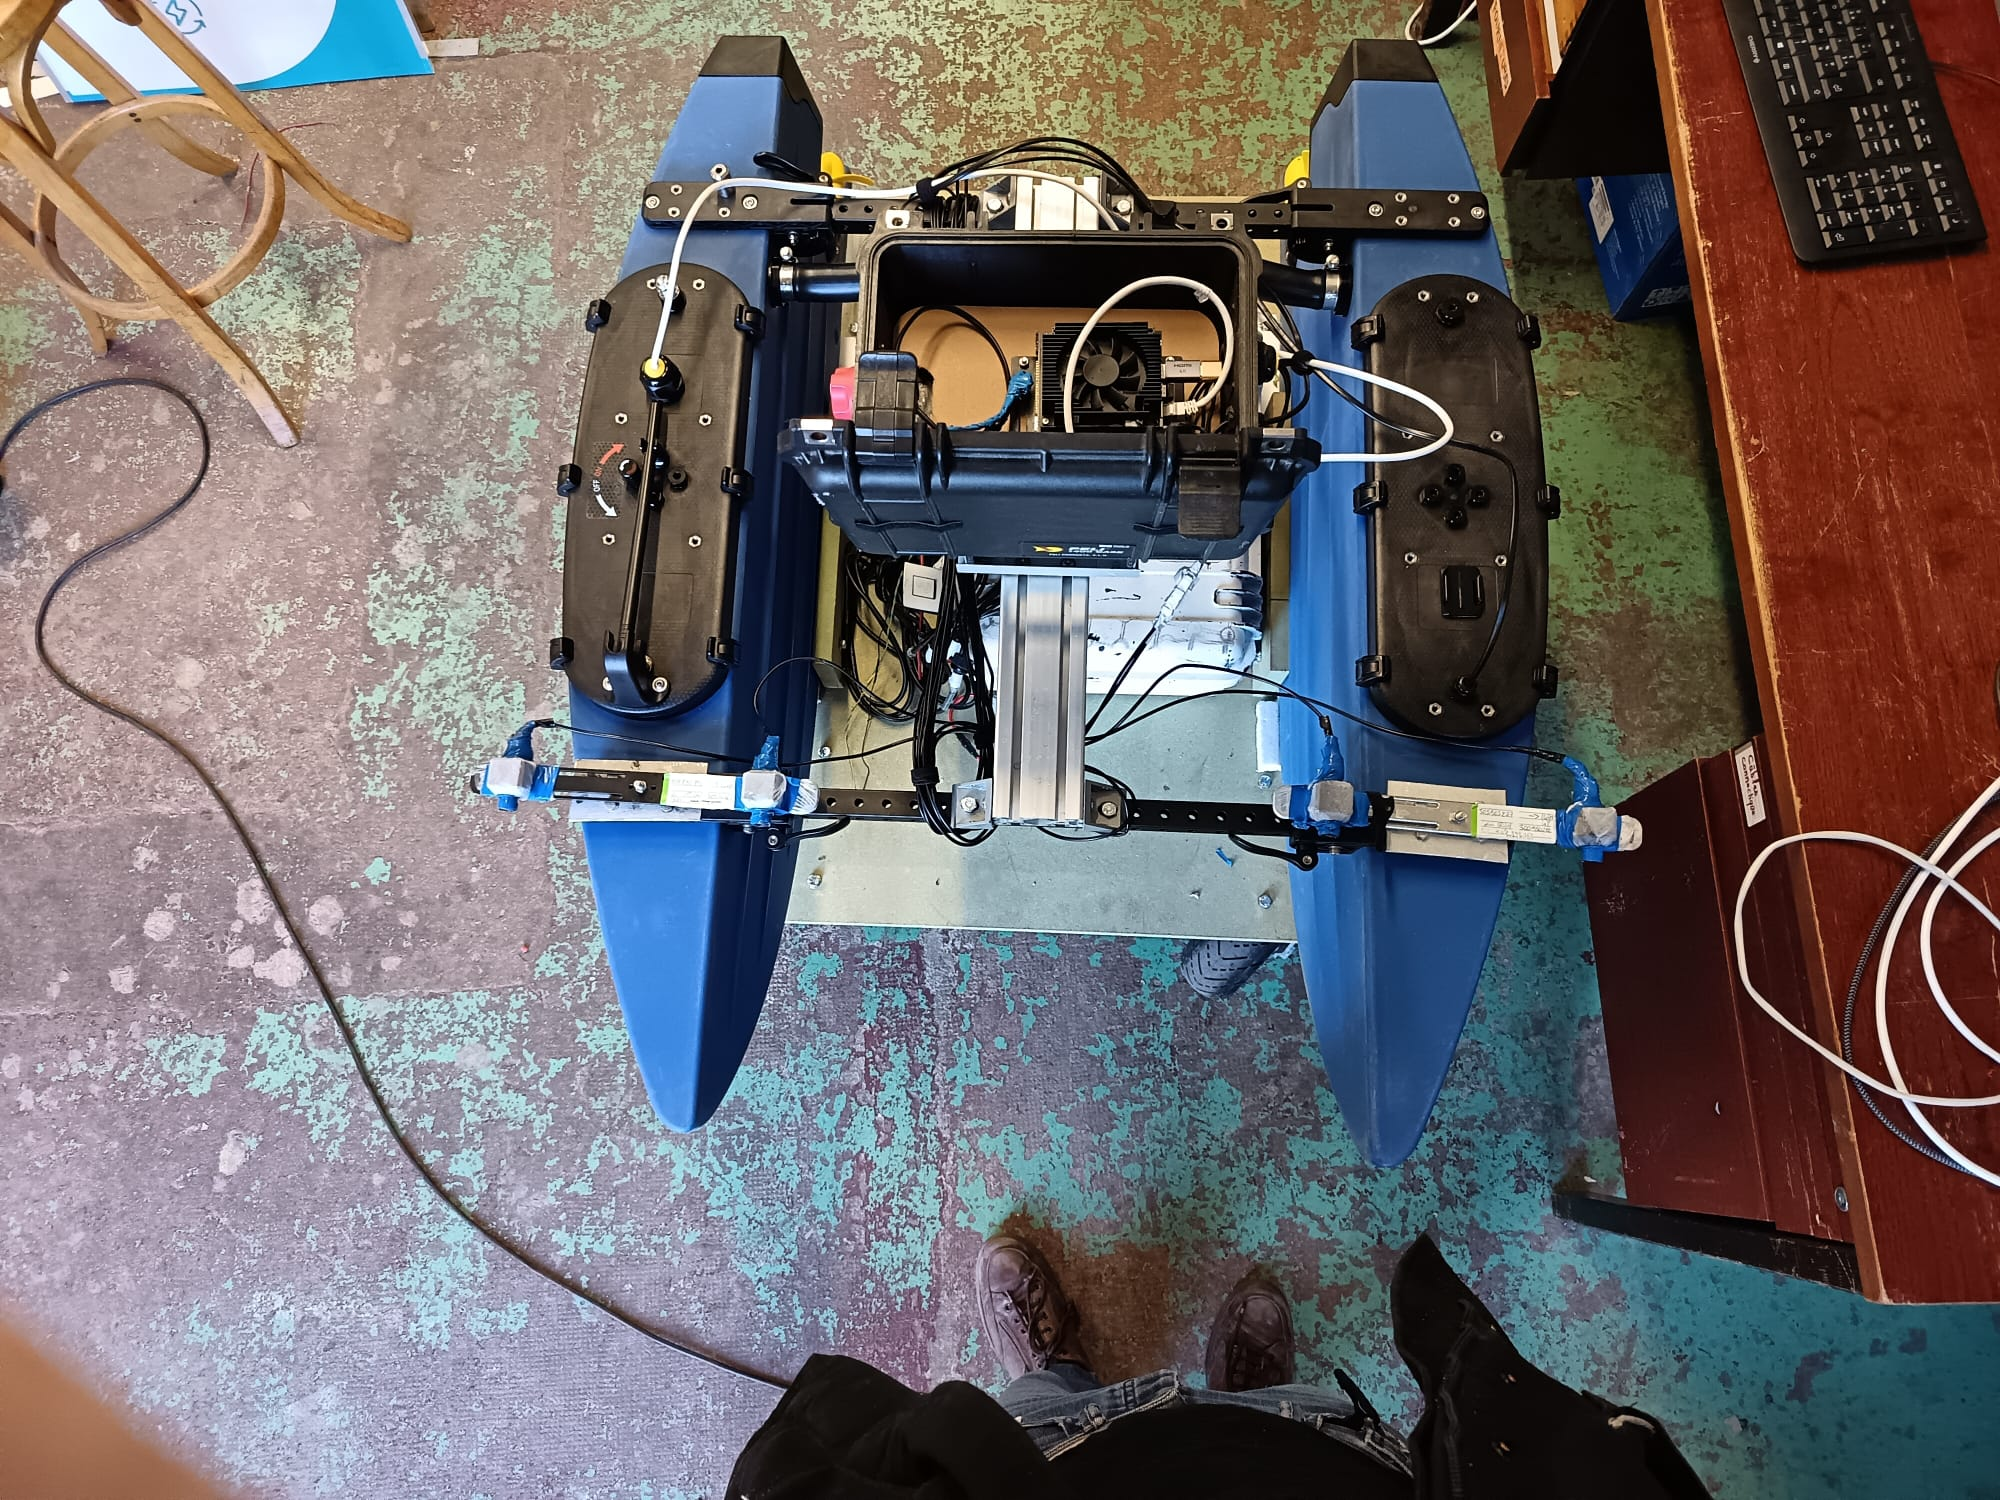
\includegraphics[width=0.75\linewidth]{blueboat-modifie.jpeg}
    \caption{BlueBoat modifié avec l'intégration du matériel nécessaire au système autonome.}
\end{figure}

\begin{figure}[H]
    \centering
    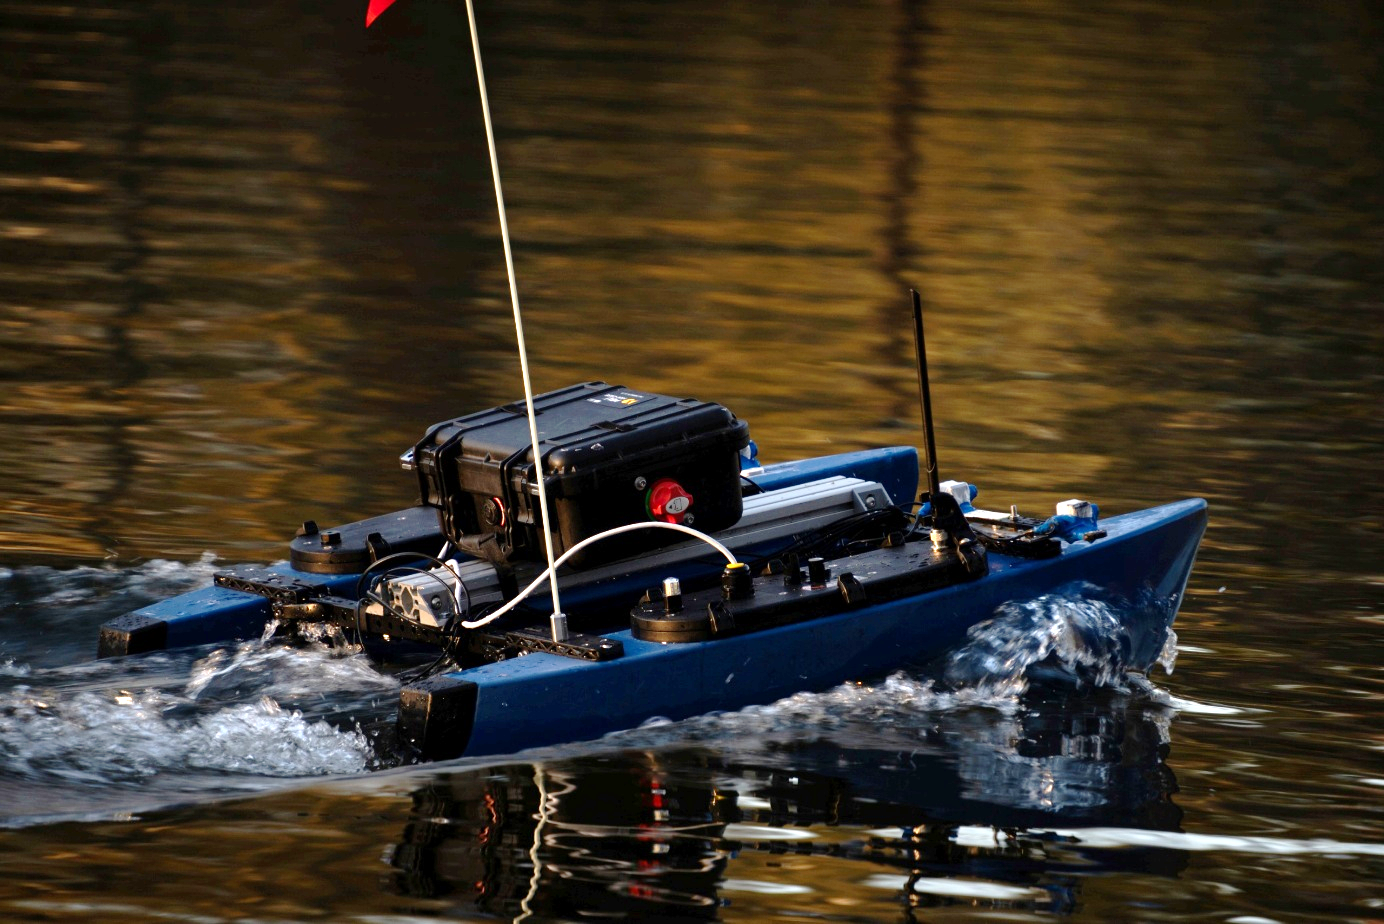
\includegraphics[width=0.75\linewidth]{bateau-final.png}
    \caption{BlueBoat équipé de son système de navigation autonome.}
\end{figure}

\subsection{Manuel d'utilisation}

Un manuel d'utilisation du BlueBoat modifié a été réalisé afin de faciliter la prise en main du système. Il regroupe une explication du fonctionnement du BlueBoat et des modifications apportées, des tutoriels pour allumer le BlueBoat et la Jetson, se connecter au BlueBoat, se connecter à la Jetson et utiliser QGroundControl. Il contient également des exemples de code propres permettant de contrôler le BlueBoat depuis la station de base.

Ce manuel constitue un livrable important, car il réduit la dépendance à une connaissance orale du système et facilite la continuité du projet pour les prochains utilisateurs.

\section{Réalisation du pôle Vision}

\subsection{Objectif du module}

Le groupe Vision a travaillé sur la partie perception du projet. L'objectif du module est de permettre au bateau autonome d'identifier les éléments utiles à la navigation maritime, principalement les bouées fixes, les bouées mobiles et les repères liés au docking. Les informations produites par ce module doivent ensuite servir de base exploitable pour les modules de décision et de trajectoire.

Le travail réalisé couvre l'ensemble de la chaîne de perception : préparation de l'environnement, constitution d'un jeu de données, annotation, entraînement d'un modèle de détection, essais d'inférence, export et préparation de l'intégration sur Jetson avec les caméras ZED.

\subsection{Mise en place de l'environnement}

La première étape a consisté à préparer un environnement de développement reproductible. Le module Vision a été organisé autour des éléments nécessaires à un pipeline complet : acquisition caméra, préparation des données, entraînement, test, export et documentation.

Des procédures d'installation ont été préparées pour Linux, Windows et Jetson. Le cas de la Jetson a demandé une attention particulière, car l'installation devait tenir compte de la version de JetPack, de CUDA, de PyTorch, de Torchvision, d'Ultralytics YOLO, du SDK ZED et des drivers nécessaires aux caméras ZED X One. L'objectif était de réduire les erreurs de configuration et de rendre le démarrage du module plus fiable sur le matériel embarqué.

\subsection{Collecte et préparation des données}

Le travail sur les données a commencé par la collecte d'images et de vidéos de scènes maritimes. Les images recherchées devaient couvrir plusieurs situations : bouées proches et lointaines, scènes avec reflets, variations de luminosité, angles de vue différents, arrière-plans maritimes et éléments associés au docking.

Le nombre d'images propres disponibles au départ était limité. Pour compenser ce manque, l'équipe a réalisé une recherche importante d'images similaires et de données maritimes disponibles en ligne. Ces images ont ensuite été triées afin de ne conserver que les cas utiles à l'apprentissage du modèle.

Dans l'état mesuré du travail, les résultats d'entraînement portent sur deux classes de bouées : \texttt{buoy\_dynamic} et \texttt{buoy\_fixed}. Le docking a été traité comme un travail d'annotation et de préparation, mais il n'est pas présenté comme une classe entraînée avec des métriques validées.

\subsection{Annotation avec CVAT}

L'annotation a été réalisée avec CVAT afin de produire des labels exploitables par YOLO. Les objets annotés comprenaient les bouées fixes, les bouées mobiles et les éléments utiles au docking. Les règles d'annotation ont été pensées pour rester simples et cohérentes : boîte englobante serrée autour de l'objet visible, annotation des objets partiellement visibles lorsqu'ils restaient identifiables, et attention particulière aux objets trop petits ou aux reflets.

Ce travail a permis d'homogénéiser des données issues de sources différentes. Les images n'avaient pas toutes la même résolution, le même angle de vue ni la même qualité. La vérification des labels a donc été une étape importante avant l'entraînement.

\subsection{Entraînement du modèle}

Une fois les données préparées, l'équipe a entraîné un modèle YOLO26 avec une politique d'augmentation adaptée aux scènes maritimes. Les augmentations avaient pour objectif d'améliorer la robustesse du modèle face aux variations de lumière, aux reflets, au bruit, au flou de mouvement et aux changements d'échelle.

Deux entraînements principaux ont été conservés pour la détection. Le second entraînement, nommé \texttt{yolo26\_maritime2}, est celui qui obtient les meilleurs résultats mesurés. Un test rapide de segmentation a aussi été mené afin de vérifier la faisabilité d'un pipeline de segmentation, même si la validation principale du rapport concerne la détection de bouées.

\subsection{Inférence, export et essais}

Après l'entraînement, des essais d'inférence ont été réalisés sur des images et des vidéos de test. Ces essais ont permis de vérifier visuellement la cohérence des boîtes prédites, la stabilité des détections et la confiance du modèle.

L'export du modèle a également été étudié afin de préparer l'utilisation embarquée. Cette étape est importante pour la Jetson, car le format du modèle et le mode d'inférence influencent directement la latence, la consommation mémoire et la compatibilité avec l'environnement GPU.

\subsection{Résultats de détection et de segmentation}

Les tests menés ont permis de vérifier l'évolution du modèle et de comparer les performances des entraînements disponibles. Les métriques utilisées sont la précision, le rappel, le mAP50 et le mAP50-95. Le mAP50 mesure la qualité des détections avec un seuil d'intersection sur union de 0,50, tandis que le mAP50-95 est plus strict puisqu'il agrège plusieurs seuils.

\begin{table}[H]
    \centering
    \caption{Comparaison des principaux entraînements de détection}
    \begin{tabular}{L{5.6cm}rrrrr}
        \toprule
        Exécution & Époque & Précision & Rappel & mAP50 & mAP50-95 \\
        \midrule
        \texttt{yolo26\_maritime} & 76 & 0,98240 & 0,94806 & 0,97830 & 0,84984 \\
        \texttt{yolo26\_maritime}, meilleur mAP50-95 & 57 & 0,98065 & 0,92424 & 0,97605 & 0,86214 \\
        \texttt{yolo26\_maritime2} & 80 & 0,99461 & 0,96994 & 0,99253 & 0,86547 \\
        \texttt{yolo26\_maritime2}, meilleur mAP50-95 & 100 & 0,98160 & 0,97282 & 0,99079 & 0,88753 \\
        \bottomrule
    \end{tabular}
\end{table}

Le second entraînement est le meilleur résultat de détection observé. Il atteint un mAP50 de 0,99253 et un mAP50-95 de 0,88753. Cela montre que le modèle détecte correctement les bouées du jeu de données actif et qu'il progresse par rapport au premier entraînement.

\begin{table}[H]
    \centering
    \caption{Test rapide de segmentation}
    \begin{tabular}{L{5.4cm}rrrr}
        \toprule
        Exécution & Époques & mAP50(B) & mAP50-95(B) & mAP50(M) \\
        \midrule
        \texttt{smoke\_test\_segmentation} & 5 & 0,97726 & 0,73281 & 0,89798 \\
        \bottomrule
    \end{tabular}
\end{table}

Le test rapide de segmentation a validé la possibilité d'exécuter un entraînement court sur une tâche plus complexe. Il ne remplace pas la validation principale de détection, mais il confirme que l'environnement peut aussi lancer ce type de modèle.

\begin{table}[H]
    \centering
    \caption{Résumé des prédictions du meilleur modèle}
    \begin{tabular}{L{4.8cm}rrrr}
        \toprule
        Modèle & Prédictions & Score moyen & Score min. & Score max. \\
        \midrule
        \texttt{yolo26\_maritime2} & 467 & 0,93135 & 0,26184 & 0,97259 \\
        \bottomrule
    \end{tabular}
\end{table}

Les prédictions du meilleur modèle présentent un score moyen de 0,93135 sur 467 prédictions. Les scores faibles isolés correspondent aux cas plus difficiles, par exemple lorsque l'objet est petit, partiellement visible ou placé dans une scène plus complexe.

Ces résultats valident principalement la détection des deux classes de bouées mesurées. Ils ne doivent pas être interprétés comme une validation quantitative du docking, qui a été travaillé au niveau de l'annotation et de la préparation, mais pas mesuré comme classe entraînée dans les résultats disponibles.

\subsection{Gestion de configuration}

La gestion de configuration du module Vision est documentée dans le manuel de configuration du module Vision. Ce manuel regroupe les prérequis matériels, les dépendances logicielles, l'installation sur les différents systèmes, la vérification des caméras ZED, l'utilisation du module et le dépannage courant.

Cette documentation est importante pour reproduire l'environnement, diagnostiquer les erreurs fréquentes et conserver une trace claire des choix techniques. Elle complète le rapport d'activité en décrivant les commandes et procédures opérationnelles nécessaires au déploiement du module.

\subsection{Difficultés du pôle Vision}

La principale difficulté a été le manque d'images initiales pour entraîner un modèle d'intelligence artificielle robuste. Les images propres de bouées et de scènes de docking étaient peu nombreuses, ce qui limitait la diversité du jeu de données. L'équipe a donc effectué une recherche importante d'images similaires et de données maritimes disponibles en ligne, puis a trié ces images, vérifié leur pertinence et adapté les annotations au format attendu.

Une autre difficulté a été la cohérence des annotations. Les bouées peuvent être petites, partiellement cachées, reflétées dans l'eau ou observées sous des angles très différents. Les éléments de docking peuvent aussi varier fortement selon les quais et les conditions de prise de vue. L'annotation avec CVAT a donc demandé de fixer des règles simples et de vérifier les labels pour éviter d'introduire du bruit dans l'entraînement.

La mise en place sur Jetson a également été complexe. Il ne suffisait pas d'installer les dépendances Python classiques : il fallait faire correspondre les versions de JetPack, CUDA, PyTorch, Torchvision, Ultralytics, le SDK ZED et les drivers des caméras. Enfin, le passage de l'entraînement à l'inférence embarquée a demandé de penser à la fois au modèle, au format exporté, aux caméras, aux performances et à la reproductibilité de l'environnement.

\section{Réalisation du pôle Embarqué}

\subsection{Objectifs et contraintes}

L'objectif principal du pôle Embarqué était l'intégration du système de contrôle avec les composants physiques du bateau, afin de garantir un système fonctionnel et testé pour la compétition. Le pôle devait assurer la communication entre les couches logicielles, les capteurs, les actionneurs et les contrôleurs, tout en gardant une architecture compatible avec les exigences de sécurité et de reprise en main.

La contrainte majeure a été l'accès tardif au châssis physique du bateau final. En conséquence, les efforts se sont concentrés sur la viabilité de la transition des fonctionnalités développées sur le BlueBoat vers le prototype final. Le BlueBoat a été utilisé comme banc d'essai pour simuler et valider les algorithmes de contrôle ainsi que la communication logicielle en parallèle de la construction du châssis officiel.

\subsection{Recherche et étude de marché}

La première étape a consisté en une recherche et une étude de marché sur les différents contrôleurs disponibles. Ce benchmarking a inclus une analyse de viabilité technique, de difficulté d'intégration et de budget.

La méthodologie de validation s'est appuyée sur les exigences de performance de la compétition, les contraintes d'étanchéité et le budget disponible. Cette analyse comparative a conduit au choix de conserver BlueOS et l'architecture ArduPilot. Ce choix est justifié par la modularité de BlueOS, sa base solide sur ArduPilot et le fait que l'équipe disposait déjà d'une carte compatible, ce qui optimisait les ressources financières et techniques.

Cette première étape a duré environ trois semaines.

\subsection{Analyse de viabilité de communication}

La deuxième étape a porté sur les tests de communication, les interfaces disponibles et les difficultés techniques associées. Les essais ont été menés sur le BlueBoat et sur le moteur disponible.

Un point critique a été identifié : le moteur sélectionné pour ses performances ne possédait pas de support natif pour communiquer avec le firmware choisi. Après arbitrage, il a été décidé de maintenir ce moteur malgré l'absence de compatibilité immédiate, en allouant du temps au développement d'une interface de communication personnalisée.

Cette étape a duré environ quatre semaines.

\subsection{Intégration des composants}

La phase d'intégration des composants a consisté à préparer les adaptations nécessaires pour le châssis final et à organiser l'intégration du moteur ainsi que des périphériques validés précédemment. Cette phase assure la transition concrète des acquis du BlueBoat vers la structure finale.

Une fois les intégrations sur le BlueBoat terminées, l'équipe a commencé à intégrer les capteurs du bateau réel sur celui-ci afin de faciliter la phase d'intégration finale. Le choix a été de conserver les capteurs déjà présents sur le BlueBoat, notamment les capteurs inertiels de la carte Navigator, à l'exception du GPS. Pour le bateau final, un GPS IP67 a été choisi afin de pouvoir le placer à l'extérieur de la boîte électrique, où il serait moins parasité. Les caméras retenues pour le bateau réel sont les mêmes que celles installées sur le BlueBoat.

\subsection{Intégration des VESC}

Les moteurs utilisés sur le bateau IA sont contrôlés par des VESC. Ils utilisent une technologie de communication différente de celle des moteurs du BlueBoat : UART pour les VESC, contre PWM dans l'architecture initiale. De plus, ArduPilot ne prévoit pas directement l'intégration de tels contrôleurs moteurs dans la configuration retenue.

Cette incompatibilité a forcé l'équipe à créer un code d'interface directement sur BlueOS afin de pouvoir contrôler le bateau tout en gardant les fonctionnalités d'ArduPilot. Le processus a été complexe, car BlueOS compartimente les données et ne permet pas facilement de modifier la version d'ArduPilot installée.

La solution retenue consiste à utiliser un script Lua lancé au démarrage. Ce script intercepte les données envoyées vers des moteurs PWM fictifs, les traduit en commandes compréhensibles par les VESC, puis les transmet en UART via le port SERIAL1 de la carte Navigator. Pour la récupération des données moteur, le protocole inverse est utilisé : les données sont récupérées via SERIAL1 en UART, puis renvoyées sur MAVLink dans des messages spécifiques de type \texttt{named\_value\_float}.

\begin{figure}[H]
    \centering
    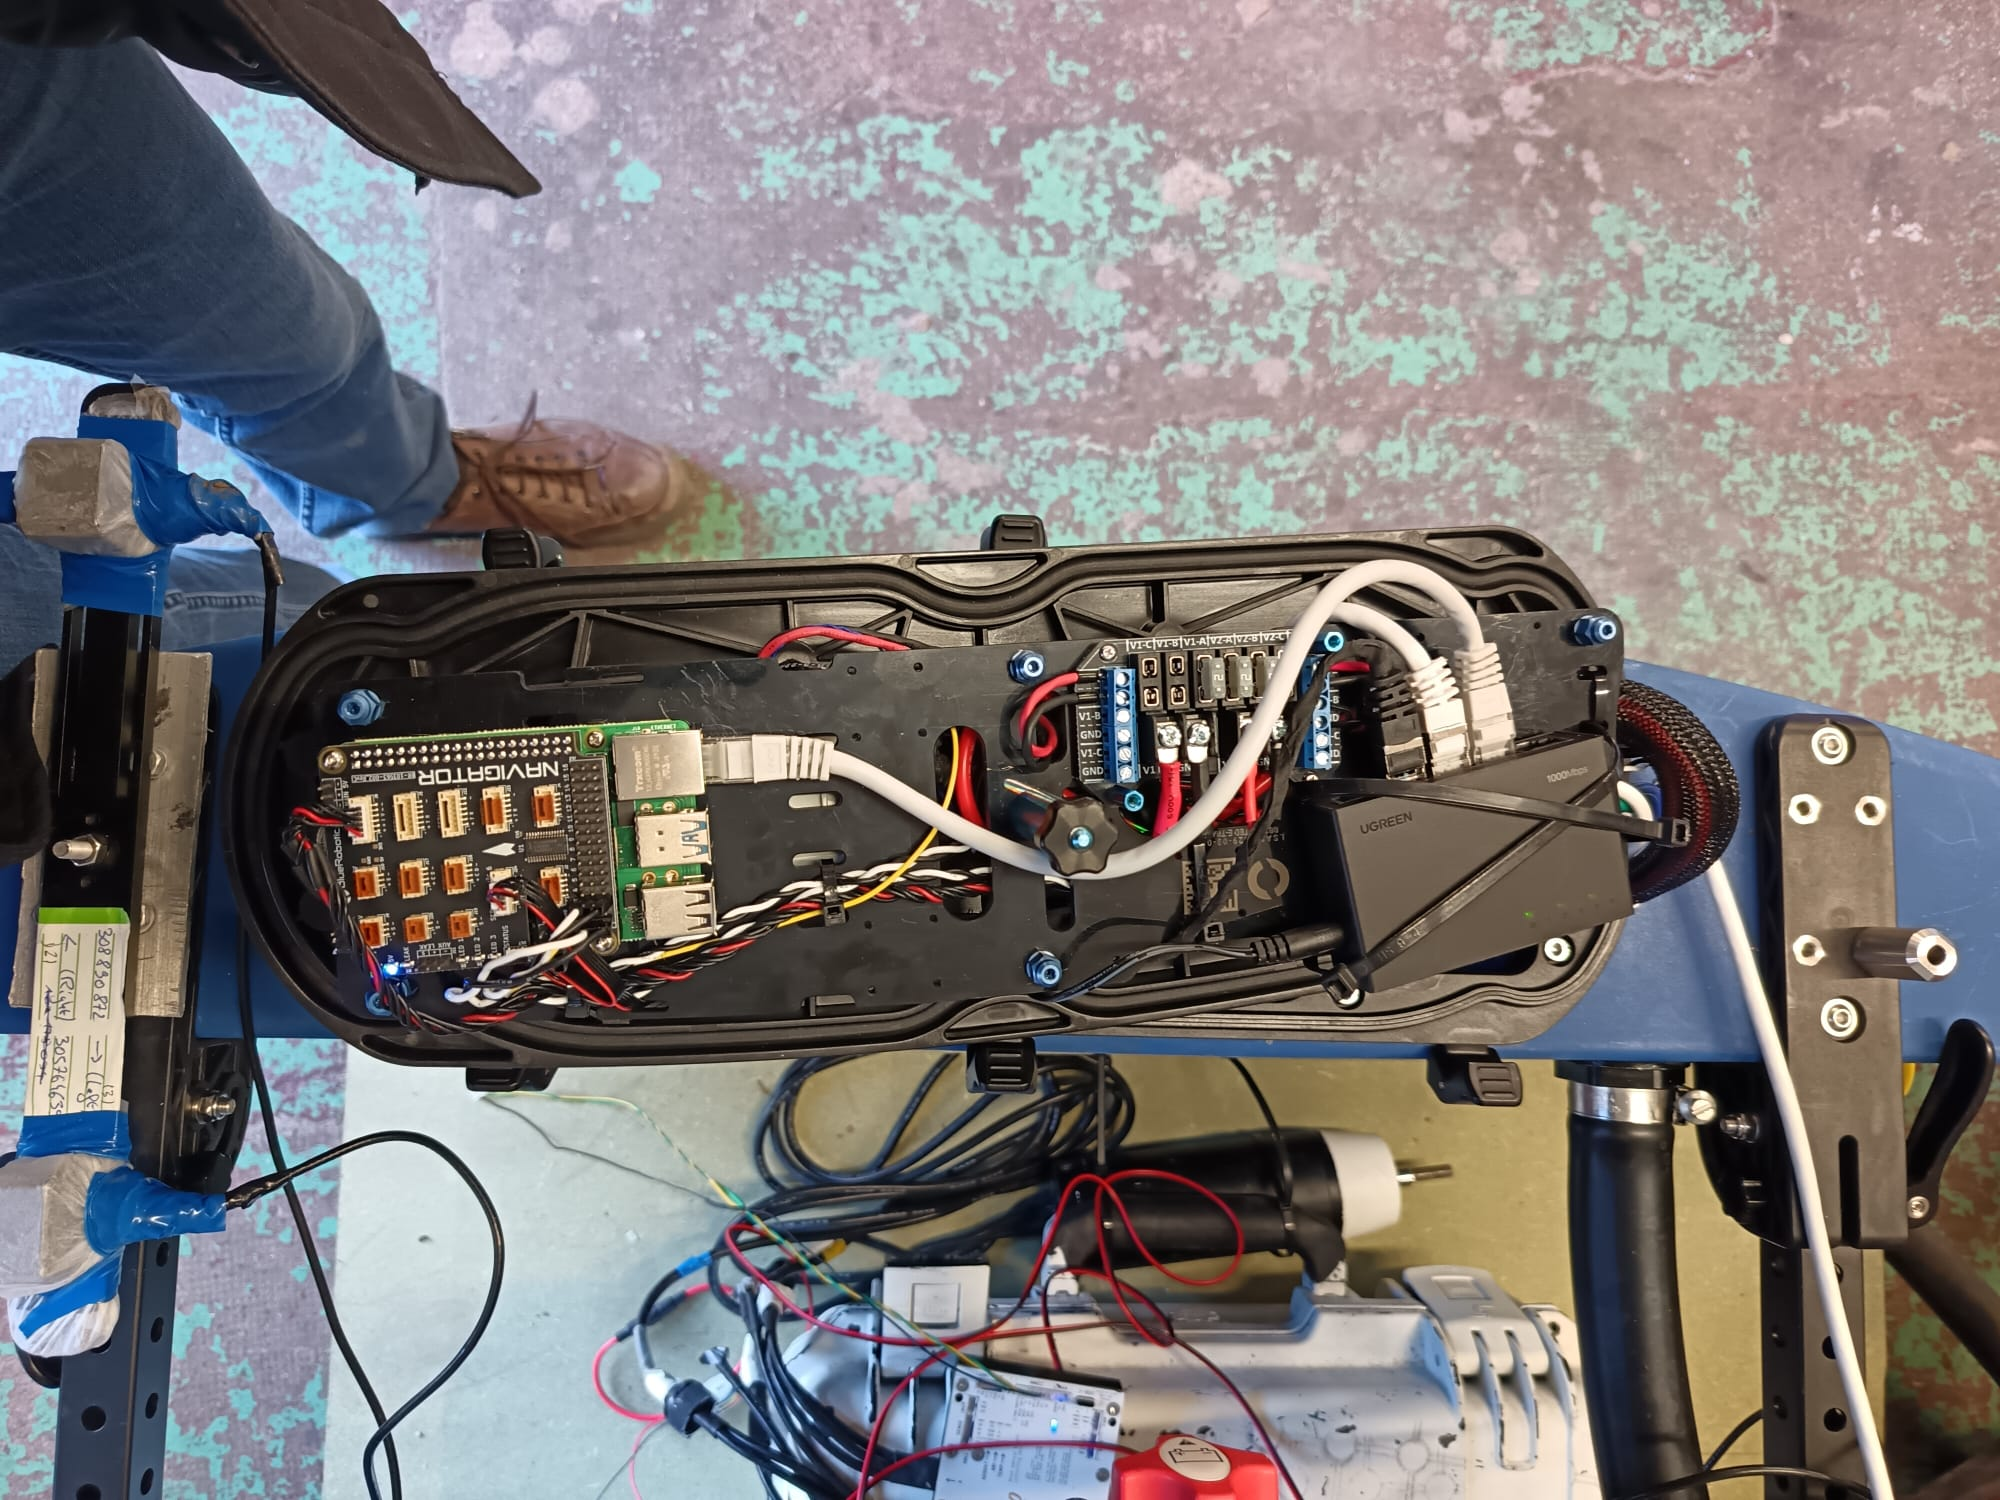
\includegraphics[width=0.72\linewidth]{blueboat-moteur.jpeg}
    \caption{Travaux d'intégration liés aux moteurs et à la transition vers les actionneurs du bateau IA.}
\end{figure}

\subsection{Tests et validation}

Les activités de tests et validation comprennent les procédures de tests finaux, l'étalonnage des capteurs et les ajustements en vue de la compétition. Les risques d'intégration avaient été cartographiés dès le début, mais leur résolution a nécessité un investissement temporel important qui a impacté le calendrier global.

Les difficultés principales du pôle Embarqué ont été la compatibilité logicielle entre BlueOS et les VESC, l'interopérabilité matérielle avec le moteur et la complexité de l'intégration des nouveaux composants sur le châssis officiel.

\section{Réalisation du pôle Intégration et Tests}

\subsection{Mission du pôle}

Le pôle Intégration et Tests a été chargé de rendre les développements exploitables sur une plateforme réelle. Les tâches comprenaient la familiarisation avec le BlueBoat, la modification de son architecture réseau, l'ajout de la Jetson et des caméras, le choix d'une méthode de contrôle permettant une reprise en main rapide et sécurisée, la création d'un manuel d'utilisation, les tests du code d'IA en conditions réelles et l'intégration progressive d'actionneurs et de capteurs réels.

\subsection{Ajouts physiques et support de test}

Afin d'implanter le code de vision, il a fallu fixer sur l'armature du bateau les caméras, la Jetson et leur alimentation. L'ajout du switch réseau a permis d'intégrer la Jetson dans le réseau local tout en conservant l'architecture initiale du BlueBoat.

Le BlueBoat a également été fixé sur un support mobile afin de tester la qualité GPS et certains comportements sans dépendre systématiquement de l'accès à un lac. Cette solution a réduit la fréquence nécessaire des tests sur plan d'eau et a permis de poursuivre les développements à terre.

\begin{figure}[H]
    \centering
    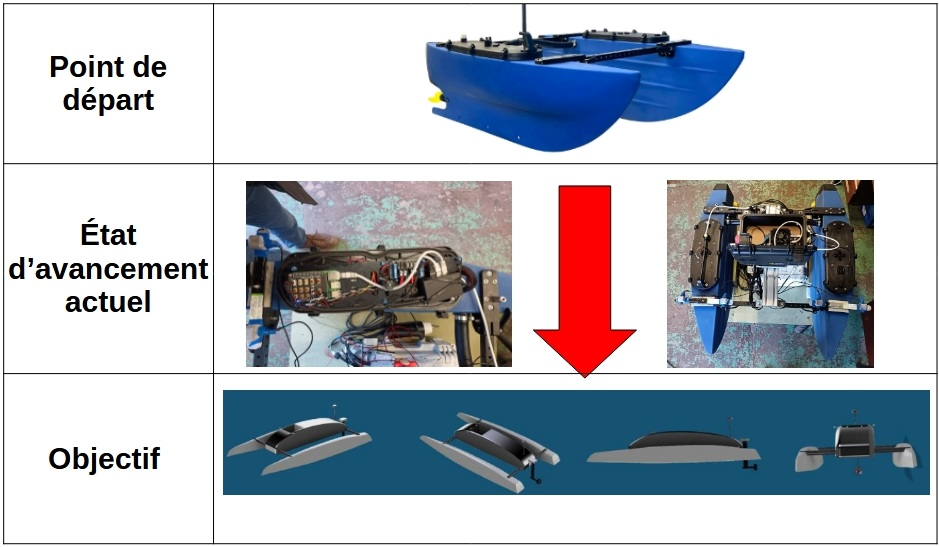
\includegraphics[width=0.75\linewidth]{etat-pie.jpg}
    \caption{État d'avancement et organisation des travaux du PIE.}
\end{figure}

\subsection{Tests du code IA et sécurité}

L'intégration du code d'IA sur une plateforme réelle impose de conserver une capacité de reprise en main. QGroundControl a été retenu notamment parce qu'il permet de visualiser la position du bateau et de changer rapidement de mode de fonctionnement. Cette capacité est importante lors des essais en conditions réelles, où le bateau doit pouvoir être repris manuellement ou placé dans un mode sûr si la partie autonome ne se comporte pas comme prévu.

Les tests ont porté sur les communications entre les modules, les commandes envoyées via MAVLink, l'accès à la Jetson, la supervision depuis la station à terre et la capacité à préparer l'intégration des composants du bateau réel.

\subsection{Livrables du pôle Intégration}

Les livrables identifiés pour ce pôle sont le manuel d'utilisation du BlueBoat, déjà rendu, le rapport PIE, ainsi qu'un guide d'exploitation pour le pilote prévu au 21 avril 2026. Ces documents complètent les développements techniques en donnant les procédures nécessaires pour utiliser et exploiter le système.

À l'état d'avancement décrit, la phase d'intégration de l'IA au BlueBoat est terminée. L'équipe se trouve au niveau de l'intégration des actionneurs et capteurs réels au BlueBoat afin de simuler le bateau réel. Il reste l'intégration du moteur de direction, de la radiocommande, ainsi que les tests et ajustements sur le bateau réel.

\section{Réalisation du pôle Conception du bateau réel}

\subsection{Contribution à la conception globale}

En collaboration avec les étudiants de première année de l'association TAMEO, une contribution a été apportée à la conception du bateau réel destiné à participer aux courses de Monaco au mois de juillet. Cette phase avait pour objectif de définir une architecture cohérente et réaliste du système, en tenant compte des contraintes techniques et des ressources disponibles.

Le choix de la plateforme nautique s'est orienté vers un Hobie Cat 14 d'occasion comme base du projet. Ce choix s'est appuyé sur des critères de stabilité, de disponibilité et d'adéquation avec les contraintes du challenge. En parallèle, le châssis en aluminium a été conçu en s'inspirant largement de celui développé pour le bateau de la classe Energy de l'association. Cette approche a permis de capitaliser sur un retour d'expérience existant tout en adaptant la structure aux spécificités du nouveau bateau.

\begin{figure}[H]
    \centering
    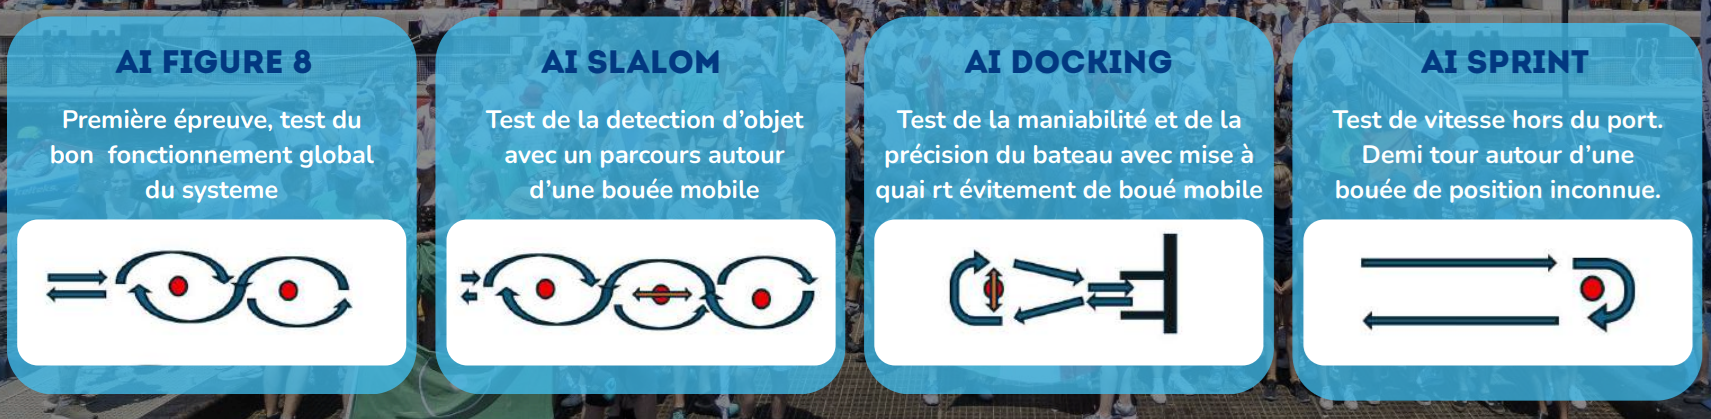
\includegraphics[width=0.9\linewidth]{ia-courses.png}
    \caption{Cadre de compétition du projet bateau IA.}
\end{figure}

\subsection{Architecture électrique}

La conception du système électrique global a été menée en cohérence avec les besoins du nouveau bateau. L'architecture repose sur une batterie principale déjà utilisée lors de précédentes compétitions, intégrée dans une configuration adaptée aux besoins du projet IA. Le reste du circuit électrique a été défini en veillant à assurer la cohérence entre les différents sous-systèmes, leur alimentation et leur intégration dans le bateau.

L'intégration de la Jetson sur le BlueBoat a également servi de retour d'expérience pour le bateau final : alimentation fiable, boîte étanche, câblage sécurisé, contraintes de centre de gravité et communication réseau sont autant de points qui ont alimenté la conception globale.

\subsection{Étude du système de direction}

Le système de direction constituait un enjeu critique du projet, car il s'agissait de la première mise en place d'un système de direction entièrement électrique sur un bateau de l'association. L'un des verrous principaux résidait dans l'estimation des efforts hydrodynamiques appliqués au safran lors des phases de manœuvre, afin de dimensionner correctement le moteur ainsi que le système d'entraînement associé.

Le choix s'est orienté vers un moteur brushless couplé à un contrôleur permettant un asservissement en position. Cette solution offre une meilleure précision dans le pilotage du safran, condition nécessaire pour envisager à terme un contrôle autonome fiable de la trajectoire du bateau.

En parallèle, une réflexion a été menée sur la conception du safran. Une modification importante a consisté à repositionner l'axe de rotation vers le centre de la surface du safran. Cette évolution permet de réduire le couple exercé par l'eau, de limiter les efforts à fournir par le système de direction et d'améliorer l'efficacité globale du dispositif.

À ce stade du projet, l'architecture du système de direction est validée. La fabrication du nouveau safran est en cours de finalisation par les étudiants de première année, et des essais en conditions réelles sont prévus afin de valider les choix effectués.

\subsection{Vérification de la conformité au règlement}

La conformité au règlement du challenge a constitué un point de vigilance important tout au long du projet, d'autant plus que la catégorie IA n'en est qu'à sa seconde édition. Les règles ont évolué de manière significative au cours de l'année, ce qui a nécessité une adaptation continue.

Pendant plusieurs mois, il a été envisagé de supprimer complètement la présence d'un pilote à bord, au profit d'un contrôle exclusivement à distance en dehors des phases de course. Cette orientation a finalement été abandonnée au profit d'un système hybride permettant à la fois la présence d'un pilote et un contrôle via radiocommande, notamment pour les phases de mise en place sur la ligne de départ.

Ces évolutions ont fait l'objet de nombreuses réunions à distance avec les organisateurs et ont impliqué des ajustements réguliers dans la conception du bateau. Le cahier des charges du challenge étant particulièrement détaillé, il a été consulté régulièrement afin de s'assurer que les choix techniques restaient conformes aux exigences imposées.

\subsection{Conception de bancs de test}

Afin de permettre aux étudiants travaillant sur la partie informatique d'avancer en parallèle du développement du bateau, plusieurs bancs de test ont été conçus et mis en place. L'objectif était de tester les composants électroniques sélectionnés, de valider leur fonctionnement et de permettre leur prise en main logicielle avant leur intégration sur le bateau final.

Dans une logique de continuité avec les développements réalisés sur le BlueBoat, il a été décidé de conserver le même contrôleur pour le bateau réel afin de faciliter le passage à l'échelle. Un banc de test a donc été conçu pour connecter le moteur principal du futur bateau au contrôleur du BlueBoat, en utilisant une alimentation indépendante. Ce dispositif a permis à l'équipe informatique de développer et tester les commandes moteur directement via l'environnement logiciel existant du BlueBoat.

Un travail similaire a été réalisé pour le système de direction. Le moteur de direction a été intégré à un banc de test spécifique, connecté lui aussi au contrôleur du BlueBoat via un câblage et une alimentation adaptés. Plusieurs autres composants, tels qu'un GPS secondaire et le système de radiocommande, ont également été intégrés à ces bancs de test. Ces dispositifs ont permis de vérifier leur fonctionnement et leur compatibilité avec l'architecture existante, tout en offrant un environnement de test à terre fiable avant l'intégration définitive sur le bateau.

\section{Gestion technique et logistique}

La gestion technique du projet ne s'est pas limitée à la conception et à l'intégration. En tant que directeur technique de l'association TAMEO (Loup COUERRE), un suivi du budget global a été assuré. Ce budget couvrait à la fois le projet de bateau autonome, le développement de l'autre bateau engagé en classe Energy, les besoins liés au fonctionnement général de l'association et la participation au challenge.

La gestion des achats nécessaires à l'avancement du projet a inclus le suivi des financements issus des sponsors et leur allocation aux différents pôles. Une organisation a été mise en place pour effectuer des commandes régulières, parfois plusieurs fois par semaine, afin de répondre rapidement aux besoins des équipes et d'éviter les blocages.

La réception et le suivi des colis ont également été pris en charge, avec une attention portée au respect des délais annoncés par les fournisseurs. La mise à disposition rapide des composants auprès des équipes a contribué à maintenir un rythme de travail efficace et à limiter les interruptions liées aux contraintes logistiques.

\section{Difficultés rencontrées et solutions apportées}

Les difficultés rencontrées ne concernent pas un seul pôle. Elles relèvent à la fois de la disponibilité des données, de la compatibilité logicielle, de l'intégration physique, du règlement, de la logistique et de la transition entre plateforme de test et bateau réel.

\begin{longtable}{L{2.5cm}L{3.8cm}L{3.8cm}L{4cm}}
    \caption{Synthèse transversale des difficultés et solutions}\\
    \toprule
    Type & Difficulté & Impact & Solution ou réponse apportée \\
    \midrule
    \endfirsthead
    \toprule
    Type & Difficulté & Impact & Solution ou réponse apportée \\
    \midrule
    \endhead
    Vision & Manque d'images initiales de bouées et de docking & Jeu de données peu diversifié et entraînement moins robuste & Recherche de données maritimes en ligne, tri des images, annotation CVAT et constitution progressive d'un dataset exploitable \\
    Vision & Cohérence des annotations difficile à maintenir & Risque d'introduire du bruit dans l'entraînement & Règles d'annotation simples, boîtes serrées, annotation des objets partiellement visibles lorsqu'ils sont identifiables, vérification des labels \\
    Vision & Installation Jetson complexe & Risques d'incompatibilité entre dépendances & Prise en compte conjointe de JetPack, CUDA, PyTorch, Torchvision, Ultralytics, SDK ZED et drivers des caméras ZED X One \\
    Embarqué & Compatibilité BlueOS et VESC & Les moteurs retenus ne sont pas supportés nativement par l'architecture choisie & Développement d'une interface spécifique avec script Lua, interception des commandes PWM fictives et traduction vers les VESC en UART \\
    Embarqué & Communication moteur non native avec le firmware choisi & Risque de devoir changer de moteur ou d'architecture & Maintien du moteur pour ses performances et allocation de temps au développement d'une interface personnalisée \\
    Intégration & Ajout de la Jetson et des caméras sur le BlueBoat & Contraintes d'étanchéité, d'alimentation, de fixation et de centre de gravité & Boîte étanche mobile, supports caméra, câblage électrique dédié et intégration au réseau par switch Ethernet \\
    Intégration & Manque de points d'eau facilement accessibles & Tests réels plus difficiles à organiser & Création d'une plateforme mobile pour tester certains comportements et la qualité GPS à terre \\
    Intégration & Manque de documentation spécifique au BlueBoat modifié & Difficulté de reprise du système par d'autres utilisateurs & Création d'un manuel d'utilisation avec explications, tutoriels de connexion, QGroundControl et exemples de code \\
    Bateau réel & Accès tardif au châssis final & Risque de bloquer les développements logiciels et l'intégration & Utilisation du BlueBoat comme banc d'essai et conception de bancs de test pour actionneurs, GPS et radiocommande \\
    Bateau réel & Dimensionnement du système de direction électrique & Incertitude sur les efforts hydrodynamiques appliqués au safran & Choix d'un moteur brushless avec asservissement en position et repositionnement de l'axe du safran pour réduire le couple \\
    Règlement & Évolution des règles de la catégorie IA & Adaptations régulières du châssis et du mode de pilotage & Suivi du cahier des charges, réunions avec les organisateurs et adoption d'un système hybride pilote/radiocommande \\
    Logistique & Besoins matériels fréquents et dépendance aux fournisseurs & Risque de blocage des équipes & Suivi du budget, commandes régulières, réception des colis et mise à disposition rapide des composants \\
    \bottomrule
\end{longtable}

\section{État d'avancement, livrables et conclusion}

\subsection{État d'avancement}

À la date de ce dossier, les bases nécessaires à la perception du BlueBoat sont en place : environnement de développement, installation multi-plateforme, configuration Jetson, collecte et annotation des données, entraînement YOLO26, premiers exports et tests d'inférence. Les résultats de détection montrent une détection fiable des bouées du jeu de données actif.

La phase d'intégration de l'IA au BlueBoat est terminée. Le réseau, l'ajout de la Jetson, les caméras, l'accès distant, l'utilisation de QGroundControl et les communications MAVLink ont été mis en place. L'intégration des actionneurs et capteurs réels sur le BlueBoat est engagée afin de simuler le bateau final et de préparer la transition.

Sur le bateau réel, les choix structurants ont été réalisés : plateforme Hobie Cat 14, châssis aluminium, architecture électrique, direction brushless asservie en position, évolution du safran, bancs de test pour le moteur principal, le moteur de direction, le GPS secondaire et la radiocommande. La conformité réglementaire continue d'être suivie en fonction des évolutions du challenge.

\subsection{Livrables}

Les livrables identifiés sont les suivants :

\begin{itemize}
    \item manuel d'utilisation du BlueBoat modifié ;
    \item rapport PIE et dossier de réalisation ;
    \item manuel de configuration du module Vision ;
    \item pipeline Vision avec données, annotations, entraînements, tests d'inférence et préparation de l'export ;
    \item architecture réseau BlueBoat, Jetson, caméras et station à terre ;
    \item scripts et logique d'interface pour l'intégration des VESC via BlueOS, ArduPilot, Lua, UART et MAVLink ;
    \item bancs de test pour les actionneurs, la direction, le GPS et la radiocommande ;
    \item suivi de conception du bateau réel et de la conformité au règlement.
\end{itemize}

\subsection{Travaux restants}

Les prochaines étapes consistent à enrichir le jeu de données Vision avec davantage d'images réelles, à étendre les métriques aux éléments de docking lorsque les annotations seront suffisamment nombreuses, puis à poursuivre l'intégration embarquée avec les caméras ZED et les modules de navigation.

Du côté de l'intégration, il reste à finaliser l'intégration du moteur de direction et de la radiocommande, puis à réaliser les tests et ajustements sur le bateau réel. Les essais en conditions réelles devront valider le comportement du système de direction, la cohérence des commandes moteur, la fiabilité des communications et la capacité de reprise en main.

\subsection{Conclusion}

Le projet a permis de mettre en place une chaîne technique complète allant de la perception jusqu'à l'intégration physique. Malgré l'accès tardif au bateau final, le BlueBoat a permis de maintenir l'avancement des développements, de tester les communications, de préparer l'intégration de la Jetson et des caméras, et de valider une partie des choix d'architecture.

Les travaux du pôle Vision ont stabilisé un pipeline de détection de bouées avec des résultats mesurés élevés sur le jeu de données actif. Les travaux du pôle Embarqué ont permis de conserver l'architecture BlueOS et ArduPilot tout en préparant l'intégration de contrôleurs moteurs VESC non supportés nativement. Les travaux d'intégration et de conception ont assuré la transition vers le bateau réel, notamment par les bancs de test, le système de direction, l'architecture électrique et le suivi réglementaire.

L'ensemble forme une base cohérente pour poursuivre l'intégration finale du bateau autonome et préparer sa participation à la compétition.

\end{document}
